%% LyX 2.3.6.1 created this file.  For more info, see http://www.lyx.org/.
%% Do not edit unless you really know what you are doing.
\documentclass[english]{article}
\usepackage[T1]{fontenc}
\usepackage[latin9]{inputenc}
\usepackage{textcomp}
\usepackage{url}
\usepackage{amsmath}
\usepackage{graphicx}

\makeatletter

%%%%%%%%%%%%%%%%%%%%%%%%%%%%%% LyX specific LaTeX commands.
%% Because html converters don't know tabularnewline
\providecommand{\tabularnewline}{\\}

\makeatother

\usepackage{babel}
\begin{document}
\title{A rule based method to locate the bounds of neural networks}
\author{Ioannis G. Tsoulos, Alexandros Tzallas, Evangelos Karvounis}
\date{Department of Informatics and Telecommunications, University of Ioannina,
Greece}
\maketitle
\begin{abstract}
An advanced method of training artificial neural networks is presented
here, which aims to identify the optimal interval for initialization
and training of artificial neural networks. The location of the optimal
interval is performed using rules evolving from a genetic algorithm.
The method has two phases: in the first phase, an attempt is made
to locate the optimal interval and in the second phase, the artificial
neural network is initialized and trained in this interval using a
method of global optimization, such as genetic algorithms. The method
has been tested on a range of categorization and function learning
data and the experimental results are extremely encouraging.
\end{abstract}

\section{Introduction }

Artificial Neural networks (ANNs) are programming tools \cite{nn1,nn2}
based on a series of parameters that are commonly called weights or
processing units. They have been used in a variety of problems from
different scientific areas, such as physics \cite{nnphysics1,nnphysics2,nnphysics3},
solving of differential equations \cite{nnde1,nnde2}, agriculture
\cite{nnagr1,nnagr2}, chemistry \cite{nnchem1,nnchem2,nnchem3},
economics \cite{nnecon1,nnecon2,nncecon3}, medicine \cite{nnmed1,nnmed2}
etc. A common way to express a neural network is a function $N(\overrightarrow{x},\overrightarrow{w})$,
with $\overrightarrow{x}$ the input vector (commonly called pattern)
and $\overrightarrow{w}$ the weight vector. A method that trains
a neural network should be used to estimate the vector $\overrightarrow{w}$
for a certain problem. The training procedure can also be formulated
as an optimization problem, where the target is to minimize the so-called
error function:
\begin{equation}
E\left(N\left(\overrightarrow{x},\overrightarrow{w}\right)\right)=\sum_{i=1}^{M}\left(N\left(\overrightarrow{x}_{i},\overrightarrow{w}\right)-y_{i}\right)^{2}\label{eq:eq1}
\end{equation}
In equation \ref{eq:eq1} the set $\left(\overrightarrow{x_{i}},y_{i}\right),\ i=1,...,M$
is the dataset used to train the neural network, with $y_{i}$ being
the actual output for the point $\overrightarrow{x_{i}}$ . The neural
network $N(\overrightarrow{x},\overrightarrow{w})$ can be modeled
as a summation of processing units as proposed in \cite{nnc}:
\begin{equation}
N\left(\overrightarrow{x},\overrightarrow{w}\right)=\sum_{i=1}^{H}w_{(d+2)i-(d+1)}\sigma\left(\sum_{j=1}^{d}x_{j}w_{(d+2)i-(d+1)+j}+w_{(d+2)i}\right)\label{eq:nn}
\end{equation}
with $H$ is the number of processing units of the neural network
and $d$ is the dimension of vector $\overrightarrow{x}$. The function$\sigma(x)$
is the sigmoid function defined as: 
\begin{equation}
\sigma(x)=\frac{1}{1+\exp(-x)}\label{eq:sig}
\end{equation}
From the equation \ref{eq:nn} one can obtain that the dimension of
the weight vector $w$ is computed as: $n=(d+2)H$. The function of
equation \ref{eq:eq1} has been minimized with a variety of optimization
methods during the past years such as: the Back Propagation method
\cite{bpnn,bpnn2}, the RPROP method \cite{rpropnn,rpropnn3,rpropnn2},
Quasi Newton methods \cite{quasinn,quasinn2}, Simulated Annealing
\cite{nn_ann1,nn_ann2}, Genetic Algorithms \cite{geneticnn,geneticnn2},
Particle Swarm Optimization \cite{psonn,psonn2} etc. Also, various
researchers have worked on the initialization of the weights of the
neural networks such as initialization using decision trees \cite{weight_init1},
an initialization method based on the Cauchy's inequality \cite{weight_init2},
a method based on discriminant learning \cite{weight_init3} etc.
Another topic that attracted the interest of many researchers is the
weight decaying, which is a regularization method that adapts the
weights of the network aiming to avoid the overfitting problem.\textbf{
}Several papers have appeared in this area such as method with positive
correlation \cite{weight_decay1}, the SarProp algorithm \cite{weight_decay2},
incorporation of pruning techniques \cite{weight_decay3} etc. Also,
more advanced and more recent techniques from the area of computational
intelligence have been proposed for neural network training such as
the Differential Evolution method \cite{weight_de1,weight_de2}, construction
of neural networks with Ant Colony Optimization \cite{weight_aco},
construction of neural networks using Grammatical Evolution to solve
differential equations \cite{weight_nnc} etc. Furthermore, due to
development of GPU units a lot of works have been published that take
advantage of these processing units \cite{weight_gpu1,weight_gpu2}.

The present work proposes an innovative interval generation technique
for the initialization and training of artificial neural network parameters.
This new method has its roots in interval methods \cite{interval0,interval1,interval2}.
In current work, using arithmetic intervals, a set of rules for dividing
the initial interval for the parameters of the artificial neural network
is constructed. The construction is carried out using a hybrid genetic
algorithm, in which chromosomes are the set of division rules. After
the termination of the genetic algorithm, the artificial neural network
is initialized in the interval resulting from the application of the
optimal partitioning rules and then trained using a genetic algorithm.\textbf{ }

This method used has two objectives: the first objective is to detect
a small interval of initialization of the parameters of the artificial
neural network and the second objective is to accelerate the training
of the network. In the first target, using information from the training
data the algorithm will make an attempt to identify that interval
that will ultimately give better results. In the second objective,
once a small value interval has been detected, a global optimization
method can be used more efficiently to detect the lowest value of
the network error.

The proposed method is expected to achieve significant results since
in principle it has all the advantages of genetic algorithms, such
as tolerance on errors, possibilities for parallel implementation,
efficient exploration of the research space, etc. In addition, in
the first phase of the method will reduce the volume of the possible
values for the weights, so that in the second phase the search for
global minimum of the network error function becomes more efficient
and faster.

The proposed methodology can even be applied to different types of
artificial neural networks such as Recurrent Neural networks \cite{rnn1,rnn2}.
A simple recurrent neural network can be expressed as single neural
cell with a single input, a single output and a state (also known
as the memory of the cell). Given the input of the cell $x(t)$ at
step $t$ and the previous state of the cell $h(t-1)$ at step $t-1$
the updated state of the cell $h(t)$ is estimated as shown in the
equation: 
\begin{equation}
\textbf{h}(t)=f\left(\textbf{W}_{hh}*\textbf{h}(t-1)+\textbf{W}_{xh}*\textbf{x}(t)+\textbf{b}_{h}\right)
\end{equation}

\begin{equation}
\boldsymbol{y}(t)=\sigma\left(\boldsymbol{W}_{hy}\text{\textasteriskcentered}h(t)+\boldsymbol{b}_{y}\right)
\end{equation}
where the $f(x)$ function is usually the softmax function. The proposed
method can be used here to estimate a promising bounding box for the
vector parameters $\textbf{W},\textbf{b}$ of the network before any
other training method is applied. 

The rest of this article is as follows:\textbf{ }in section \ref{sec:Method-description}
the proposed method is discussed in detail, in section \ref{sec:Experiments}
the experimental datasets as well as the results from the application
of the proposed method are provided and finally in section \ref{sec:Conclusions}
some conclusions and guidelines for future enhancements are presented.

\section{Method description \label{sec:Method-description}}

The proposed method consists of two major steps: in the first step,
the construction of the partition rules of the initial value interval
for the parameters of the artificial neural network is made and in
the second step, the artificial neural network is initialized in the
optimal space resulting from the first step and training takes place.
The training is performed through a second genetic algorithm. In the
first genetic algorithm, the chromosomes are sets of partition rules
of the initial value interval of the artificial neural network, and
in the second genetic algorithm, the chromosomes are the parameters
of the artificial neural network. It is obvious that this is a time
consuming process and modern parallel techniques such as the OpenMP
\cite{openmp} library must be used to accelerate it. The first genetic
algorithm is analyzed in subsection \ref{subsec:Locating-the-best}
and the second in subsection \ref{subsec:Training-of-the}.

\subsection{Locating the best rules \label{subsec:Locating-the-best}}

Firstly, we introduce the rule set $I_{n}$ where:
\begin{equation}
I_{n}=\left\{ \left(l_{1},r_{1}\right),\left(l_{2},r_{2}\right),\ldots,\left(l_{n},r_{n}\right)\right\} \label{eq:I_eq}
\end{equation}
where $l_{i}\in\left\{ 0,1\right\} ,\ r_{i}\in\left\{ 0,1\right\} ,\ i=1,\ldots,n$.
The set $I_{n}$ defines the set of partition rules for a function
defined as 
\begin{equation}
f:S\rightarrow R,S\subset R^{n}\label{eq:f_eq}
\end{equation}
with $S$: 
\begin{equation}
S=\left[a_{1},b_{1}\right]\otimes\left[a_{2},b_{2}\right]\otimes\ldots\left[a_{n},b_{n}\right]\label{eq:eq_defines}
\end{equation}
If $l_{i}=1$ then $a_{i}=\frac{a_{i}}{2}$ and if $r_{i}=1$ then
$b_{i}=\frac{b_{i}}{2}$. For example consider the Rastrigin function:
\begin{equation}
f(x)=x_{1}^{2}+x_{2}^{2}-\cos\left(18x_{1}\right)-\cos\left(18x_{2}\right),\ x\in[-1,1]^{2}
\end{equation}
Also consider the set $I_{2}=\left\{ \left(1,0\right),\left(0,1\right)\right\} $
The produced bounding box for the Rastrigin function is now $S'=\left[-0.5,1\right]\times\left[-1,0.5\right]$.

Subsequently, we introduce the extended set $C_{Kn}$ as a set of
production rules defined as:
\begin{equation}
R_{Kn}=\left\{ I_{n}^{(1)},I_{n}^{(2)},\ldots,I_{n}^{(K)}\right\} \label{eq:ck}
\end{equation}
where $I_{n}^{(i)},\ i=1,..,K$ are rule sets of equation \ref{eq:I_eq}.
For example let $K=2$ for the Rastrigin function and $R_{22}=\left\{ \left\{ \left(0,1\right),\left(1,0\right)\right\} ,\left\{ \left(1,0\right),\left(1,1\right)\right\} \right\} $.
The final bounding box is considered after applying the sets $\left\{ \left(0,1\right),\left(1,0\right)\right\} $
and $\left\{ \left(1,0\right),\left(1,1\right)\right\} $ in the original
box $S$. The computation steps are:
\begin{enumerate}
\item \textbf{Apply} $\left\{ \left(0,1\right),\left(1,0\right)\right\} $to
S yielding $S'=\left[-0.5,1\right]\times\left[-1,0.5\right]$
\item \textbf{Apply} $\left\{ \left(1,0\right),\left(1,1\right)\right\} $
to $S'$ yielding $S''=\left[-0.25,1\right]\times\left[-0.5,0.25\right]$
\end{enumerate}
We consider chromosomes in the form of equation \ref{eq:ck} for the
first phase of the proposed method. The value $n$ is the total number
of parameters of the neural network. The fitness of every chromosome
$g$ is an interval $f_{g}=\left[f_{g,\mbox{min}},f_{g,\mbox{max}}\right]$.
Hence, in order to compare two different intervals $a=\left[a_{1},a_{2}\right]$
and $b=\left[b_{1},b_{2}\right]$ we incorporate the following function:
\begin{eqnarray}
L^{*}(a,b) & = & \begin{cases}
\mbox{TRUE}, & a_{1}<b_{1},\mbox{OR\ \ensuremath{\left(a_{1}=b_{1}\ \mbox{AND}\ a_{2}<b_{2}\right)}}\\
\mbox{FALSE}, & \mbox{\mbox{OTHERWISE}}
\end{cases}\label{eq:eql}
\end{eqnarray}

Hence, the steps of the genetic algorithm of the first phase are the
following:

\paragraph{Initialization step}
\begin{enumerate}
\item \textbf{Set} $K$ as the number of rules.
\item \textbf{Set} $S=\left[-D,D\right]^{n}$, as the initial bounding box
for the parameters of the neural network. $D$ is considered as a
positive number with $D>1$.
\item \textbf{Set} $N_{C}$ as the total number of chromosomes.
\item \textbf{Set} $N_{S}$ the number of samples in fitness evaluation.
\item \textbf{Set} $P_{s}$ as the selection rate, where $P_{s}\le1$.
\item \textbf{Set} $P_{m}$ as the mutation rate, where $P_{m}\le1$.
\item \textbf{Set} $t=0$ the current generation number.
\item \textbf{Set} $N_{t}$ the maximum number of generations allowed.
\item \textbf{Initialize} randomly the chromosomes $C_{i},\ i=1,..,N_{C}$
as sets of the equation \ref{eq:ck}.
\end{enumerate}

\paragraph{Termination check step }
\begin{enumerate}
\item \textbf{Set} t=t+1
\item \textbf{If} $t\ge N_{t}$ \textbf{terminate}.
\end{enumerate}

\paragraph{Genetic operations step }
\begin{enumerate}
\item \textbf{For} every chromosome $C_{i},\ i=1,..,N_{C}$ calculate the
corresponding fitness value $f_{i}$ using the algorithm of subsection
\ref{subsec:FitnessRule}.
\item \textbf{Apply} the selection operator. Initially, the chromosomes
are sorted according to their fitness value. The sorting utilizes
the function $L^{*}(a,b)$ of equation \ref{eq:eql} to compare fitness
values. The best\textbf{ $\left(1-P_{s}\right)\times N_{c}$ }are
copied to the next generation\textbf{ }while the rest of them are
substituted by offsprings created through the crossover procedure.
The mating parents for the crossover procedure are selected using
the well - known technique of tournament selection.
\item \textbf{Apply} the crossover operator: For every pair of selected
parents $(z,w),$ two children $(cz,cw)$ are produced using the uniform
crossover procedure described in subsection \ref{subsec:CrossoverRule}.
\item \textbf{Apply} the mutation operator using the algorithm of subsection
\ref{subsec:MutationRule}.
\item \textbf{Goto} Termination Check Step. 
\end{enumerate}

\subsection{Fitness evaluation for the rule genetic algorithm\label{subsec:FitnessRule}}

The fitness value for each chromosome $g$ is considered as an interval
$f=\left[f_{\mbox{min}},f_{\mbox{max}}\right]$ where $f_{\mbox{min}}$is
an estimation of the lower value obtained using the rules of the chromosome
$g$ and $f_{\mbox{max}}$is an estimation of the maximum value. In
order to calculate the fitness of every set of rules $C$ the following
steps are performed:
\begin{enumerate}
\item \textbf{Set} $f_{\mbox{min}}=\infty$
\item \textbf{Set} $f_{\mbox{max}}=-\infty$
\item \textbf{Apply} the rule set $g$ to the original bounding box $S$.
The outcome of this application is the new bounding box $S_{g}$.
\item \textbf{For} $i=1,..,N_{S}$ \textbf{do}
\begin{enumerate}
\item \textbf{Produce} a random sample $w\in S_{g}$
\item \textbf{Calculate} the training error $E_{g}=E\left(N\left(\overrightarrow{x},\overrightarrow{w}\right)\right)$
using equation \ref{eq:eq1}.
\item \textbf{If} $E_{g}\le f_{\mbox{min}}$ then $f_{\mbox{min}}=E_{g}$.
\item \textbf{If} $E_{g}\ge f_{max}$ then $f_{\mbox{max}}=E_{g}$.
\end{enumerate}
\item \textbf{EndFor}
\item \textbf{Return} the interval $f=\left[f_{\mbox{min}},f_{\mbox{max}}\right]$
as the fitness of chromosome $g.$
\end{enumerate}

\subsection{Crossover for the rule genetic algorithm\label{subsec:CrossoverRule}}

The crossover for the genetic algorithm of the first phase is performed
using uniform crossover. For every couple $(z,w)$ of selected parents
two children $(cz,cw)$ are produced through the following procedure:
\begin{enumerate}
\item \textbf{For} $i=1..K$ \textbf{do}
\begin{enumerate}
\item \textbf{Let} $z^{(i)}=\left\{ l_{z}^{(i)},r_{z}^{(i)}\right\} $ the
$i$ item of the chromosome $z$.
\item \textbf{Let} $w^{(i)}=\left\{ l_{w}^{(i)},r_{w}^{(i)}\right\} $ the
$i$ item of the chromosome $w$.
\item \textbf{Produce} a random number $r\le1$
\item \textbf{If} $r\le0.5$ \textbf{then} 
\begin{enumerate}
\item \textbf{Set} $\mbox{cz}^{(i)}=\left\{ l_{z}^{(i)},r_{w}^{(i)}\right\} $
\item \textbf{Set} $\mbox{cw}^{(i)}=\left\{ l_{w}^{(i)},r_{z}^{(i)}\right\} $
\end{enumerate}
\item \textbf{Else}
\begin{enumerate}
\item \textbf{Set} $\mbox{cz}^{(i)}=\left\{ l_{w}^{(i)},r_{z}^{(i)}\right\} $
\item \textbf{Set} $\mbox{cw}^{(i)}=\left\{ l_{z}^{(i)},r_{w}^{(i)}\right\} $
\end{enumerate}
\item \textbf{Endif}
\end{enumerate}
\item \textbf{EndFor}
\end{enumerate}

\subsection{Mutation for the rule genetic algorithm\label{subsec:MutationRule}}

The steps for the mutation procedure for the genetic algorithm of
the first phase have as following:
\begin{enumerate}
\item \textbf{For} $i=1,..,N_{C}$ \textbf{do}
\begin{enumerate}
\item \textbf{Let} $C_{i}=\left\{ C_{i}^{(1)},C_{i}^{(2)},\ldots,C_{i}^{(K)}\right\} $
the i chromosome of the population.
\item \textbf{For} $j=1,..,K$ \textbf{do}
\begin{enumerate}
\item \textbf{Let} $C_{i}^{(j)}=\left\{ l_{i}^{(j)},r_{i}^{(j)}\right\} $
\item \textbf{Take} $r\le$1 a random number.
\item \textbf{If} $r\le P_{m}$ \textbf{then} alter randomly with probability
50\% the $l_{i}^{(j)}$ or the $r_{i}^{(j)}$ part of $C_{i}^{(j)}$.
\end{enumerate}
\item \textbf{EndFor}
\end{enumerate}
\item \textbf{EndFor}
\end{enumerate}

\subsection{Second phase\label{subsec:Training-of-the}}

In the second phase the best chromosome $g_{b}$ defined as 
\begin{equation}
g_{\mbox{b}}=\left\{ \left\{ l_{b,1},r_{b,1}\right\} ,\left\{ l_{b,2},r_{b,2}\right\} ,\ldots,\left\{ l_{b,K},r_{b,K}\right\} \right\} 
\end{equation}
 is used to transform the original bounding box $S=[-F,F]^{(n)}$
to a new box $S_{b}$. The new hyperbox is defined as 
\begin{equation}
S_{b}=\left[a_{g,1},b_{g,1}\right]\times\left[a_{g,2},b_{g,2}\right]\times\ldots\times\left[a_{g,n},b_{g,n}\right]
\end{equation}
This hyperbox will be used to bound the parameters of the neural network.
The parameters of the network are trained using a genetic algorithm
with the following steps:

\paragraph{Initialization step}
\begin{enumerate}
\item \textbf{Set} $N_{C}$ as the total number of chromosomes.
\item \textbf{Set} $P_{s}$ as the selection rate, where $P_{s}\le1$.
\item \textbf{Set} $P_{m}$ as the mutation rate, where $P_{m}\le1$.
\item \textbf{Set} $t=0$ the current generation number.
\item \textbf{Set} $N_{t}$ the maximum number of generations allowed.
\item \textbf{Initialize} randomly the chromosomes $C_{i},\ i=1,..,N_{C}$
inside the bounding box $S_{b}$. 
\end{enumerate}

\paragraph{Termination check step }
\begin{enumerate}
\item \textbf{Set} t=t+1
\item \textbf{If} $t\ge N_{t}$ \textbf{goto} Local Search Step.
\end{enumerate}

\paragraph{Genetic operations step }
\begin{enumerate}
\item \textbf{Calculate} the fitness value of every chromosome
\begin{enumerate}
\item \textbf{For} $i=1..N_{C}$ \textbf{Do}
\begin{enumerate}
\item \textbf{Set} $f_{i}=E\left(N\left(\overrightarrow{x},C_{i}\right)\right)$
using the equation \ref{eq:eq1}\@.
\end{enumerate}
\item \textbf{EndFor}
\end{enumerate}
\item \textbf{Apply} the crossover operator. In this phase the best\textbf{
$\left(1-P_{s}\right)\times N_{c}$} chromosomes are transferred intact
to the next generation. The rest of the chromosomes are substituted
by offsprings created through crossover. The selection of two parents
$x=\left(x_{1},x_{2},...,x_{n}\right),\ \ y=\left(y_{1},y_{2},...,y_{n}\right)$
for crossover is performed using tournament selection. Having selected
the parents, the offsprings $\tilde{x}$ and $\tilde{y}$ are formed
using the following:
\begin{eqnarray}
\tilde{x_{i}} & = & r_{i}x_{i}+\left(1-r_{i}\right)y_{i}\nonumber \\
\tilde{y_{i}} & = & r_{i}y_{i}+\left(1-r_{i}\right)x_{i}\label{eq:crossover_ali}
\end{eqnarray}
where $r_{i}$ are random numbers in $[-0.5,1.5]$ \cite{weight_gpu2}. 
\item \textbf{Apply} the mutation operator. The mutation scheme is the same
as in the work of Kaelo and Ali\cite{kaelo}:
\begin{enumerate}
\item \textbf{For} $i=1..N_{C}$ \textbf{do}
\begin{enumerate}
\item \textbf{For} $j=1..n$ \textbf{do}
\begin{enumerate}
\item \textbf{Let} $r\in[0,1]$ a random number
\item \textbf{If} $r\le P_{m}$ alter the element $C_{ij}$ using the following
\begin{equation}
C_{ij}=\left\{ \begin{array}{cc}
C_{ij}+\Delta\left(\mbox{t},b_{g,i}-C_{ij}\right) & t=0\\
C_{ij}-\Delta\left(\mbox{t},C_{ij}-a_{g,i}\right) & t=1
\end{array}\right.\label{eq:ali_mutation}
\end{equation}
where $t$ is a random number that takes either the values 0 or 1
and $\Delta(\mbox{t},y)$ is calculated as:
\begin{equation}
\Delta(t,y)=y\left(1-r^{\left(1-\frac{t}{N_{t}}\right)z}\right)\label{eq:delta_equation}
\end{equation}
where $r\in[0,1]$ is a random number and $z$ is a user defined parameter. 
\end{enumerate}
\item \textbf{EndFor}
\end{enumerate}
\item \textbf{EndFor}
\end{enumerate}
\item \textbf{Goto} Termination check step.
\end{enumerate}

\paragraph{Local Search step}
\begin{enumerate}
\item \textbf{Set} $C^{*}$ the best chromosome of the population.
\item \textbf{Apply} a local search procedure $C^{*}={\cal L}\left(C^{*}\right)$.
The local search procedure used was a BFGS method of Powell \cite{powell}.
\end{enumerate}

\section{Experiments \label{sec:Experiments}}

The proposed method is evaluated on a series of classification and
regression problems from the relevant literature. The classification
problems used for the experiments were found in most cases in two
internet databases:
\begin{enumerate}
\item UCI dataset repository, \url{https://archive.ics.uci.edu/ml/index.php}
\item Keel repository, \url{https://sci2s.ugr.es/keel/datasets.php}\cite{Keel}.
\end{enumerate}
The regression datasets are in most cases available from the Statlib
URL \url{ftp://lib.stat.cmu.edu/datasets/index.html }. The proposed
method is compared against a neural network trained by a genetic algorithm
and the results are reported.

\subsection{Experimental datasets }

The following classification datasets were used:
\begin{enumerate}
\item \textbf{Appendictis} a medical dataset, proposed in \cite{appendicitis}. 
\item \textbf{Australian} dataset \cite{australian}, the dataset is related
to credit card applications.
\item \textbf{Balance} dataset \cite{balance}, which is used to predict
psychological states. 
\item \textbf{Cleveland} dataset, a dataset used to detect heart disease
used in various papers\cite{cleveland1,cleveland2}.
\item \textbf{Bands} dataset, a printing problem used to identify cylinder
bands.
\item \textbf{Dermatology} dataset \cite{dermatology}, which is used for
differential diagnosis of erythemato-squamous diseases. 
\item \textbf{Hayes roth} dataset. This dataset\cite{hayesroth} contains
\textbf{5} numeric-valued attributes and 132 patterns. 
\item \textbf{Heart} dataset \cite{heart}, used to detect heart disease. 
\item \textbf{HouseVotes} dataset \cite{housevotes}, which is about votes
in the U.S. House of Representatives Congressmen. 
\item \textbf{Ionosphere} dataset. The ionosphere dataset contains data
from the Johns Hopkins Ionosphere database and it has been studied
in a bunch of papers \cite{ion1,ion2}.
\item \textbf{Liverdisorder} dataset \cite{liver}, used for detect liver
disorders in peoples using blood analysis. 
\item \textbf{Mammographic} dataset \cite{mammographic}. This dataset be
used to identify the severity (benign or malignant) of a mammographic
mass lesion from BI-RADS attributes and the patient's age. It contains
830 patterns of 5 features each.
\item \textbf{Page Blocks }dataset \cite{pageblocks}, used to detect the
page layout of a document.
\item \textbf{Parkinsons} dataset. This dataset is composed of a range of
biomedical voice measurements from 31 people, 23 with Parkinson's
disease (PD)\cite{parkinsons}.
\item \textbf{Pima} dataset \cite{pima}, used to detect the presence of
diabetes.
\item \textbf{Popfailures} dataset \cite{popfailures}, that is related
to climate model simulation crashes of simulation crashes. 
\item \textbf{Regions2} dataset. It is created from liver biopsy images
of patients with hepatitis C \cite{regions}. From each region in
the acquired images, 18 shape-based and color-based features were
extracted, while it was also annotated form medical experts. The resulting
dataset includes 600 samples belonging into 6 classes.
\item \textbf{Saheart} dataset \cite{saheart}, used to detect heart disease. 
\item \textbf{Segment} dataset \cite{segment}. This database contains patterns
from a database of 7 outdoor images (classes).
\item \textbf{Wdbc} dataset \cite{wdbc}, which contains data for breast
tumors. 
\item \textbf{Wine} dataset, used to detect through chemical analysis determine
the origin of wines and is been used in various research papers \cite{wine1,wine2}.
\item \textbf{Eeg} datasets. As an real word example, consider an EEG dataset
described in \cite{nnagr2} is used here. The dataset consists of
five sets (denoted as Z, O, N, F and S) each containing 100 single-channel
EEG segments each having 23.6 sec duration. With different combinations
of these sets the produced datasets are Z\_F\_S, ZO\_NF\_S, ZONF\_S.
\item \textbf{Zoo} dataset \cite{zoo}, where the task is classify animals
in seven predefined classes.
\end{enumerate}
Also, the following regression datasets were used:
\begin{enumerate}
\item \textbf{Abalone} dataset \cite{abalone}. This data set can be used
to obtain a model to predict the age of abalone from physical measurements. 
\item \textbf{Airfoil }dataset, which is used by the NASA for a series of
aerodynamic and acoustic tests \cite{airfoil}. 
\item \textbf{Baseball} dataset, a dataset to predict the salary of baseball
players.
\item \textbf{BK} dataset. This dataset comes from Smoothing Methods in
Statistics \cite{Stat} and is used to estimate the points scored
per minute in a basketball game. 
\item \textbf{BL} dataset: This dataset can be downloaded from StatLib.
It contains data from an experiment on the affects of machine adjustments
on the time to count bolts. 
\item \textbf{Concrete} dataset. This dataset is taken from civil engineering\cite{concrete}. 
\item \textbf{Dee} dataset, used to predict the daily average price of the
electricity energy in Spain.
\item \textbf{Diabetes} dataset, a medical dataset.
\item \textbf{Housing} dataset. This dataset was taken from the StatLib
library which is maintained at Carnegie Mellon University and it is
described in \cite{key23}.
\item \textbf{FA} dataset, which contains percentage of body fat and ten
body circumference measurements. The goal is to fit body fat to the
other measurements. 
\item \textbf{MB} dataset. This dataset is available from Smoothing Methods
in Statistics \cite{key21} and it includes 61 patterns. 
\item \textbf{MORTGAGE} dataset, which contains the Economic data information
of USA.
\item \textbf{PY }dataset, (Pyrimidines problem). The source of this dataset
is the URL: \url{https://www.dcc.fc.up.pt/~ltorgo/Regression/DataSets.html}
and it is a problem of 27 attributes and 74 number of patterns. The
task consists of Learning Quantitative Structure Activity Relationships
(QSARs) and provided by \cite{pydataset}.
\item \textbf{Quake} dataset. The objective here is to approximate the strength
of a earthquake. 
\item \textbf{Treasure} dataset, which contains Economic data information
of USA from 01/04/1980 to 02/04/2000 on a weekly basis.
\item \textbf{Wankara} dataset, which contains weather information.
\end{enumerate}

\subsection{Experimental results}

The method is compared against three other methods:
\begin{enumerate}
\item A genetic algorithm with the same parameters that are shown in Table
\ref{tab:Experimental-parameters.}. Also, after the termination of
the genetic algorithm the local search procedure of BFGS is applied
to the best chromosome of the population, in order to enhance the
quality of the solution. The column GENETIC in the experimental tables
denotes the results from the application of this method.
\item The Adam stochastic optimization method \cite{Adam} as implemented
in OptimLib, freely available from \url{https://github.com/kthohr/optim}.
The results for this method are listed in the column ADAM in the relevant
tables.
\item The Rprop method \cite{rpropnn} as implemented in the FCNN software
package \cite{fcn}. The results for this method are listed in the
column RPROP in the relevant tables.
\item The NEAT method (NeuroEvolution of Augmenting Topologies ) \cite{neat}
as implemented in EvolutionNet package freely available from \url{https://github.com/BiagioFesta/EvolutionNet}.
\end{enumerate}
All the experiments were conducted 30 times with different seeds for
the random number generator each time and averages were taken. To
perform the experiments, the software \emph{IntervalGenetic} which
is freely available from \url{https://github.com/itsoulos/IntervalGenetic}
was utilized. The experimental results for classification datasets
are shown in Table \ref{tab:Experiments-for-classification} and the
results for the regression datasets are outlined in Table \ref{tab:exp2}.
For classification problems, the average classification error on the
test set is shown and for regression datasets the average mean squared
error on the test set is displayed.\textbf{ }In all cases, 10 fold
cross validation was used and the number of hidden nodes (parameter
$H$) was set to 10. The column DATASET stands for the name of the
Dataset incorporated, the column $D=50$ represents the application
of the proposed method with $D=50$ as the initial value for the interval
of weights, the column $D=100$ stands for the results of the proposed
method with $D=100$ and finally the column $D=200$ represents the
results of the proposed method with $D=200$. In both tables, an additional
row was added at the end showing the average classification or regression
error for all datasets and it is denoted by the name AVERAGE. . All
the experiments were conducted on an AMD Ryzen 5950X equipped with
128GB of RAM. The operating system used was OpenSUSE Linux and all
the programs are compiled using the GNU C++ compiler.

As can be seen from the experimental results, the proposed method
is significantly superior than the other methods, especially in the
case of regression data. The RPROP training method seems to overcome
ADAM in most cases of classification datasets and the simple Genetic
method is better thank ADAM and RPROP for classification datasets
but not for regression datasets. Also, the change of the parameter
$D$ does not seem to have a significant effect on the performance
of the algorithm and the proposed algorithm achieves high performance
even for small values of this parameter.

In addition, the average execution times for all the problems of this
publication were compared between the proposed method and the methods
ADAM, RPROP and GENETIC mentioned above. The average execution times
are presented graphically in Figure \ref{fig:time}. In order to speed
up the proposed method, the genetic algorithm used was parallelized
using the open source library OpenMP \cite{openmp}. The column THREAD1
stands for the average time execution of the proposed method with
one thread, the column THREADS 2 represents the average execution
time of the proposed method using two threads in the OpenMP implementation,
the column THREADS 4 denotes the average execution time of the proposed
method for four threads and finally the column THREADS 8 denotes the
average execution time for eight threads for the OpenMP implementation.
The proposed method has slow execution times when performed on one
thread, but as the number of threads used increases the execution
time decreases dramatically. This is very important, because it means
that it could be used in large problems if the computer in use has
enough execution threads. Obviously all methods of training artificial
neural networks could be parallelized in one way or another. The parallelization
of the proposed method is done since it is by nature an extremely
slow method, since it requires the use of two genetic algorithms in
series. By using parallel techniques this problem is alleviated, however
the computational cost remains high. But this is the only substantial
price for using this technique. Also, a time comparison is made for
the PageBlocks dataset between the proposed method and a parallel
imlementation of the Adam algorithm named DADAM for number of threads
ranging from 1 to 8. The time comparison is graphically illustrated
in Figure \ref{fig:dadam}.

To make the dynamics of the proposed method clearer, another series
of experiments was performed. In these, the maximum number of generations
(parameter $N_{t}$) received three values: 20, 40 and 100 and for
each value all experiments for classification and regression datasets
were performed. The results for the classification datasets are listed
in Table \ref{tab:class_nt} and the results for regression datasets
are shown in Table \ref{tab:regression_nt}. As expected, the proposed
method improves its performance as the maximum number of generations
increases, but even for a small number of generations it has a satisfactory
performance.

\begin{table}
\caption{Experimental parameters.\label{tab:Experimental-parameters.}}

\begin{centering}
\begin{tabular}{|c|c|}
\hline 
PARAMETER & VALUE\tabularnewline
\hline 
\hline 
$K$ & 20\tabularnewline
\hline 
$H$ & 10\tabularnewline
\hline 
$N_{C}$ & 200\tabularnewline
\hline 
$N_{S}$ & 50\tabularnewline
\hline 
$N_{t}$ & 200\tabularnewline
\hline 
$P_{s}$ & 0.10\tabularnewline
\hline 
$P_{m}$ & 0.01\tabularnewline
\hline 
\end{tabular}
\par\end{centering}
\end{table}

\begin{table}
\caption{Experiments for classification datasets\label{tab:Experiments-for-classification}}

\centering{}%
\begin{tabular}{|c|c|c|c|c|c|c|c|}
\hline 
DATASET & GENETIC & ADAM & RPROP & NEAT & $D=50$ & $D=100$ & $D=200$\tabularnewline
\hline 
\hline 
Appendicitis & 18.10\% & 16.50\% & 16.30\% & 17.20\% & 15.00\% & 14.00\% & 16.07\%\tabularnewline
\hline 
Australian & 32.21\% & 35.65\% & 36.12\% & 31.98\% & 24.85\% & 30.20\% & 28.52\%\tabularnewline
\hline 
Balance & 8.97\% & 7.87\% & 8.81\% & 23.14\% & 7.42\% & 7.42\% & 7.67\%\tabularnewline
\hline 
Bands & 35.75\% & 36.25\% & 36.32\% & 34.30\% & 32.00\% & 32.25\% & 33.06\%\tabularnewline
\hline 
Cleveland & 51.60\% & 67.55\% & 61.41\% & 53.44\% & 41.64\% & 44.66\% & 44.39\%\tabularnewline
\hline 
Dermatology & 30.58\% & 26.14\% & 15.12\% & 32.43\% & 15.49\% & 11.00\% & 10.80\%\tabularnewline
\hline 
Hayes Roth & 56.18\% & 59.70\% & 37.46\% & 50.15\% & 28.72\% & 28.84\% & 32.05\%\tabularnewline
\hline 
Heart & 28.34\% & 38.53\% & 30.51\% & 39.27\% & 15.58\% & 17.07\% & 16.22\%\tabularnewline
\hline 
HouseVotes & 6.62\% & 7.48\% & 6.04\% & 10.89\% & 3.92\% & 3.78\% & 3.26\%\tabularnewline
\hline 
Ionosphere & 15.14\% & 16.64\% & 13.65\% & 19.67\% & 12.25\% & 9.71\% & 7.12\%\tabularnewline
\hline 
Liverdisorder & 31.11\% & 41.53\% & 40.26\% & 30.67\% & 30.90\% & 29.54\% & 30.70\%\tabularnewline
\hline 
Lymography & 23.26\% & 29.26\% & 24.67\% & 33.70\% & 18.98\% & 17.52\% & 17.67\%\tabularnewline
\hline 
Mammographic & 19.88\% & 46.25\% & 18.46\% & 22.85\% & 17.01\% & 17.60\% & 15.97\%\tabularnewline
\hline 
PageBlocks & 8.06\% & 7.93\% & 7.82\% & 10.22\% & 7.73\% & 7.01\% & 6.71\%\tabularnewline
\hline 
Parkinsons & 18.05\% & 24.06\% & 22.28\% & 18.56\% & 14.81\% & 13.86\% & 12.53\%\tabularnewline
\hline 
Pima & 32.19\% & 34.85\% & 34.27\% & 34.51\% & 23.51\% & 25.31\% & 27.49\%\tabularnewline
\hline 
Popfailures & 5.94\% & 5.18\% & 4.81\% & 7.05\% & 6.13\% & 5.93\% & 5.30\%\tabularnewline
\hline 
Regions2 & 29.39\% & 29.85\% & 27.53\% & 33.23\% & 24.01\% & 23.14\% & 23.62\%\tabularnewline
\hline 
Saheart & 34.86\% & 34.04\% & 34.90\% & 34.51\% & 28.94\% & 29.04\% & 29.93\%\tabularnewline
\hline 
Segment & 57.72\% & 49.75\% & 52.14\% & 66.72\% & 47.38\% & 49.49\% & 40.61\%\tabularnewline
\hline 
Wdbc & 8.56\% & 35.35\% & 21.57\% & 12.88\% & 6.23\% & 5.28\% & 5.49\%\tabularnewline
\hline 
Wine & 19.20\% & 29.40\% & 30.73\% & 25.43\% & 5.51\% & 6.55\% & 6.22\%\tabularnewline
\hline 
Z\_F\_S & 10.73\% & 47.81\% & 29.28\% & 38.41\% & 4.70\% & 5.61\% & 6.01\%\tabularnewline
\hline 
ZO\_NF\_S & 8.41\% & 47.43\% & 6.43\% & 43.75\% & 5.39\% & 4.67\% & 5.81\%\tabularnewline
\hline 
ZONF\_S & 2.60\% & 11.99\% & 27.27\% & 5.44\% & 1.85\% & 2.07\% & 2.24\%\tabularnewline
\hline 
ZOO & 16.67\% & 14.13\% & 15.47\% & 20.27\% & 14.83\% & 11.40\% & 8.50\%\tabularnewline
\hline 
\textbf{AVERAGE} & \textbf{23.47\%} & \textbf{30.81\%} & \textbf{25.37\%} & \textbf{28.87\%} & \textbf{17.49\%} & \textbf{17.42\%} & \textbf{17.08\%}\tabularnewline
\hline 
\end{tabular}
\end{table}

\begin{table}
\caption{Experiments for regression datasets.\label{tab:exp2}}

\centering{}%
\begin{tabular}{|c|c|c|c|c|c|c|c|}
\hline 
DATASET & GENETIC & ADAM & RPROP & NEAT & $D=50$ & $D=100$ & $D=200$\tabularnewline
\hline 
\hline 
ABALONE & 7.17 & 4.30 & 4.55 & 9.88 & 4.22 & 4.18 & 3.89\tabularnewline
\hline 
AIRFOIL & 0.003 & 0.005 & 0.002 & 0.067 & 0.003 & 0.003 & 0.003\tabularnewline
\hline 
BASEBALL & 103.60 & 77.90 & 92.05 & 100.39 & 49.47 & 51.07 & 53.57\tabularnewline
\hline 
BK & 0.027 & 0.03 & 1.599 & 0.15 & 0.017 & 0.017 & 0.019\tabularnewline
\hline 
BL & 5.74 & 0.28 & 4.38 & 0.05 & 0.0019 & 0.0016 & 0.0016\tabularnewline
\hline 
CONCRETE & 0.0099 & 0.078 & 0.0086 & 0.081 & 0.0053 & 0.0044 & 0.0042\tabularnewline
\hline 
DEE & 1.013 & 0.63 & 0.608 & 1.512 & 0.187 & 0.205 & 0.203\tabularnewline
\hline 
DIABETES & 19.86 & 3.03 & 1.11 & 4.25 & 0.31 & 0.31 & 0.29\tabularnewline
\hline 
HOUSING & 43.26 & 80.20 & 74.38 & 56.49 & 19.28 & 18.50 & 17.75\tabularnewline
\hline 
FA & 1.95 & 0.11 & 0.14 & 0.19 & 0.011 & 0.012 & 0.012\tabularnewline
\hline 
MB & 3.39 & 0.06 & 0.055 & 0.061 & 0.048 & 0.047 & 0.047\tabularnewline
\hline 
MORTGAGE & 2.41 & 9.24 & 9.19 & 14.11 & 0.57 & 0.70 & 0.53\tabularnewline
\hline 
PY & 105.41 & 0.09 & 0.039 & 0.075 & 0.016 & 0.014 & 0.014\tabularnewline
\hline 
QUAKE & 0.040 & 0.06 & 0.041 & 0.298 & 0.036 & 0.036 & 0.036\tabularnewline
\hline 
TREASURY & 2.929 & 11.16 & 10.88 & 15.52 & 0.473 & 0.677 & 0.622\tabularnewline
\hline 
WANKARA & 0.012 & 0.02 & 0.0003 & 0.005 & 0.0003 & 0.0002 & 0.0002\tabularnewline
\hline 
\textbf{AVERAGE} & \textbf{18.55} & \textbf{11.70} & \textbf{12.44} & \textbf{12.70} & \textbf{4.67} & \textbf{4.74} & \textbf{4.81}\tabularnewline
\hline 
\end{tabular}
\end{table}

\begin{figure}
\caption{Execution time comparison between the proposed algorithm and the other
mentioned methods.\label{fig:time}}

\raggedright{}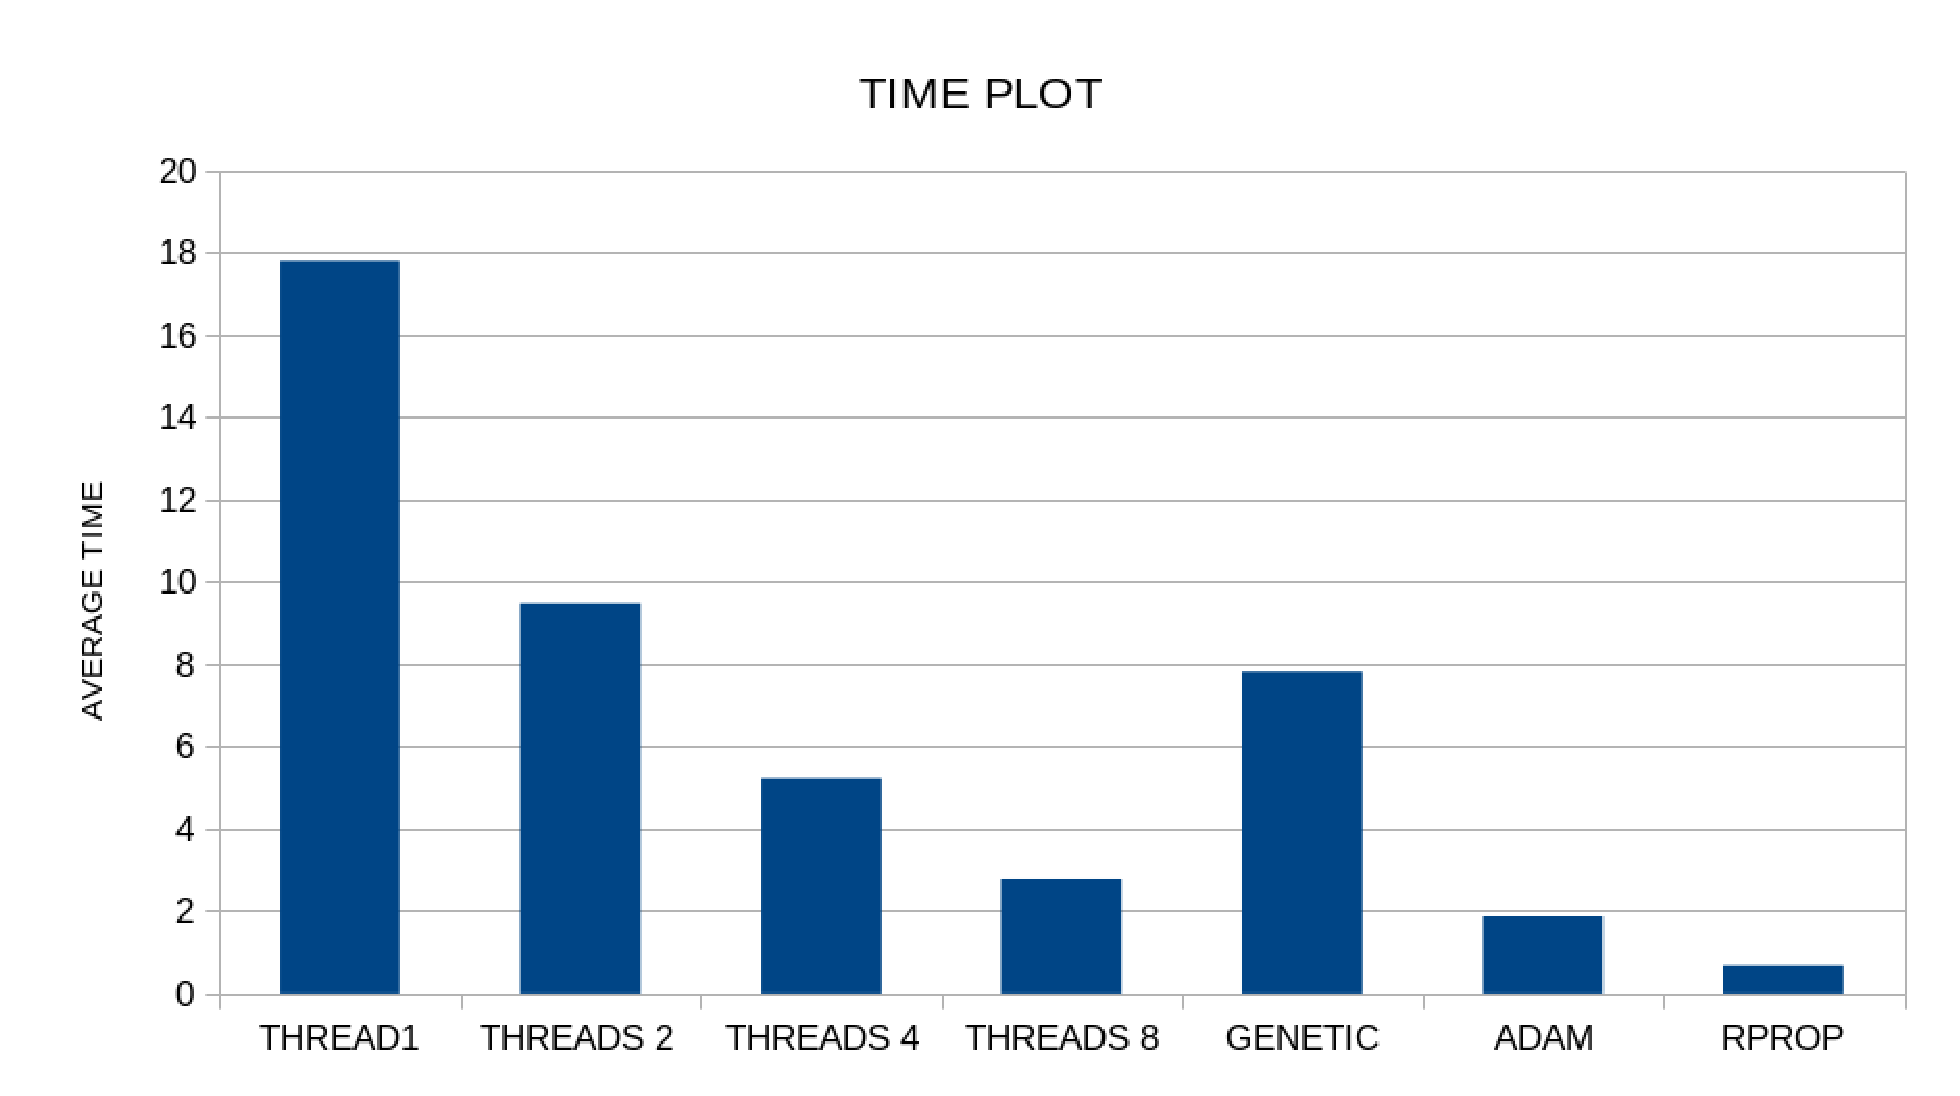
\includegraphics[scale=0.5]{time_comparison}
\end{figure}

\begin{table}
\caption{Experiments with $N_{t}$ for the classification datasets.\label{tab:class_nt}}

\begin{centering}
\begin{tabular}{|c|c|c|c|}
\hline 
DATASET & $N_{t}=20$ & $N_{t}=40$ & $N_{t}=100$\tabularnewline
\hline 
\hline 
Appendicitis & 15.23\% & 15.37\% & 15.77\%\tabularnewline
\hline 
Australian & 32.85\% & 33.15\% & 30.18\%\tabularnewline
\hline 
Balance & 11.92\% & 7.61\% & 8.71\%\tabularnewline
\hline 
Bands & 35.61\% & 33.86\% & 32.96\%\tabularnewline
\hline 
Cleveland & 43.91\% & 43.35\% & 41.29\%\tabularnewline
\hline 
Dermatology & 28.41\% & 21.28\% & 14.33\%\tabularnewline
\hline 
Hayes Roth & 50.33\% & 38.56\% & 36.80\%\tabularnewline
\hline 
Heart & 20.61\% & 21.16\% & 19.99\%\tabularnewline
\hline 
HouseVotes & 4.07\% & 4.31\% & 3.58\%\tabularnewline
\hline 
Ionosphere & 12.14\% & 11.19\% & 9.23\%\tabularnewline
\hline 
Liverdisorder & 31.47\% & 33.01\% & 31.24\%\tabularnewline
\hline 
Lymography & 22.24\% & 22.57\% & 20.74\%\tabularnewline
\hline 
Mammographic & 18.66\% & 17.37\% & 15.71\%\tabularnewline
\hline 
PageBlocks & 7.95\% & 7.68\% & 6.81\%\tabularnewline
\hline 
Parkinsons & 17.28\% & 17.44\% & 13.86\%\tabularnewline
\hline 
Pima & 33.19\% & 31.94\% & 30.71\%\tabularnewline
\hline 
Popfailures & 6.65\% & 5.81\% & 5.24\%\tabularnewline
\hline 
Regions2 & 26.33\% & 26.03\% & 22.25\%\tabularnewline
\hline 
Saheart & 36.11\% & 32.96\% & 34.45\%\tabularnewline
\hline 
Segment & 66.37\% & 58.33\% & 49.85\%\tabularnewline
\hline 
Wdbc & 7.38\% & 6.95\% & 7.68\%\tabularnewline
\hline 
Wine & 13.49\% & 11.55\% & 8.39\%\tabularnewline
\hline 
Z\_F\_S & 7.77\% & 7.59\% & 8.38\%\tabularnewline
\hline 
ZO\_NF\_S & 8.21\% & 7.52\% & 7.28\%\tabularnewline
\hline 
ZONF\_S & 2.26\% & 1.87\% & 1.99\%\tabularnewline
\hline 
ZOO & 14.70\% & 12.30\% & 13.50\%\tabularnewline
\hline 
\textbf{AVERAGE} & \textbf{22.12\%} & \textbf{20.41\%} & \textbf{18.88\%}\tabularnewline
\hline 
\end{tabular}
\par\end{centering}
\end{table}

\begin{table}

\caption{Experiments with different values of $N_{t}$ parameter for the regression
datasets.\label{tab:regression_nt}}

\begin{centering}
\begin{tabular}{|c|c|c|c|}
\hline 
DATASET & $N_{t}=20$ & $N_{t}=40$ & $N_{t}=100$\tabularnewline
\hline 
\hline 
ABALONE & 4.88 & 4.77 & 4.63\tabularnewline
\hline 
AIRFOIL & 0.004 & 0.004 & 0.004\tabularnewline
\hline 
BASEBALL & 69.83 & 65.37 & 69.72\tabularnewline
\hline 
BK & 0.02 & 0.02 & 0.02\tabularnewline
\hline 
BL & 0.006 & 0.005 & 0.007\tabularnewline
\hline 
CONCRETE & 0.008 & 0.006 & 0.005\tabularnewline
\hline 
DEE & 0.224 & 0.225 & 0.199\tabularnewline
\hline 
DIABETES & 0.357 & 0.343 & 0.321\tabularnewline
\hline 
HOUSING & 26.43 & 25.88 & 20.65\tabularnewline
\hline 
FA & 0.019 & 0.019 & 0.017\tabularnewline
\hline 
MB & 0.05 & 0.05 & 0.05\tabularnewline
\hline 
MORTGAGE & 2.11 & 1.76 & 1.44\tabularnewline
\hline 
PY & 0.02 & 0.018 & 0.022\tabularnewline
\hline 
QUAKE & 0.042 & 0.037 & 0.037\tabularnewline
\hline 
TREASURY & 2.37 & 2.12 & 1.48\tabularnewline
\hline 
WANKARA & 0.0004 & 0.0003 & 0.0003\tabularnewline
\hline 
\textbf{AVERAGE} & \textbf{6.65} & \textbf{6.29} & \textbf{6.16}\tabularnewline
\hline 
\end{tabular}
\par\end{centering}
\end{table}

\begin{figure}

\caption{Time comparison between the proposed method and a parallell implementation
of Adam algorithm. The comparison is made for the dataset Page Blocks.\label{fig:dadam}}

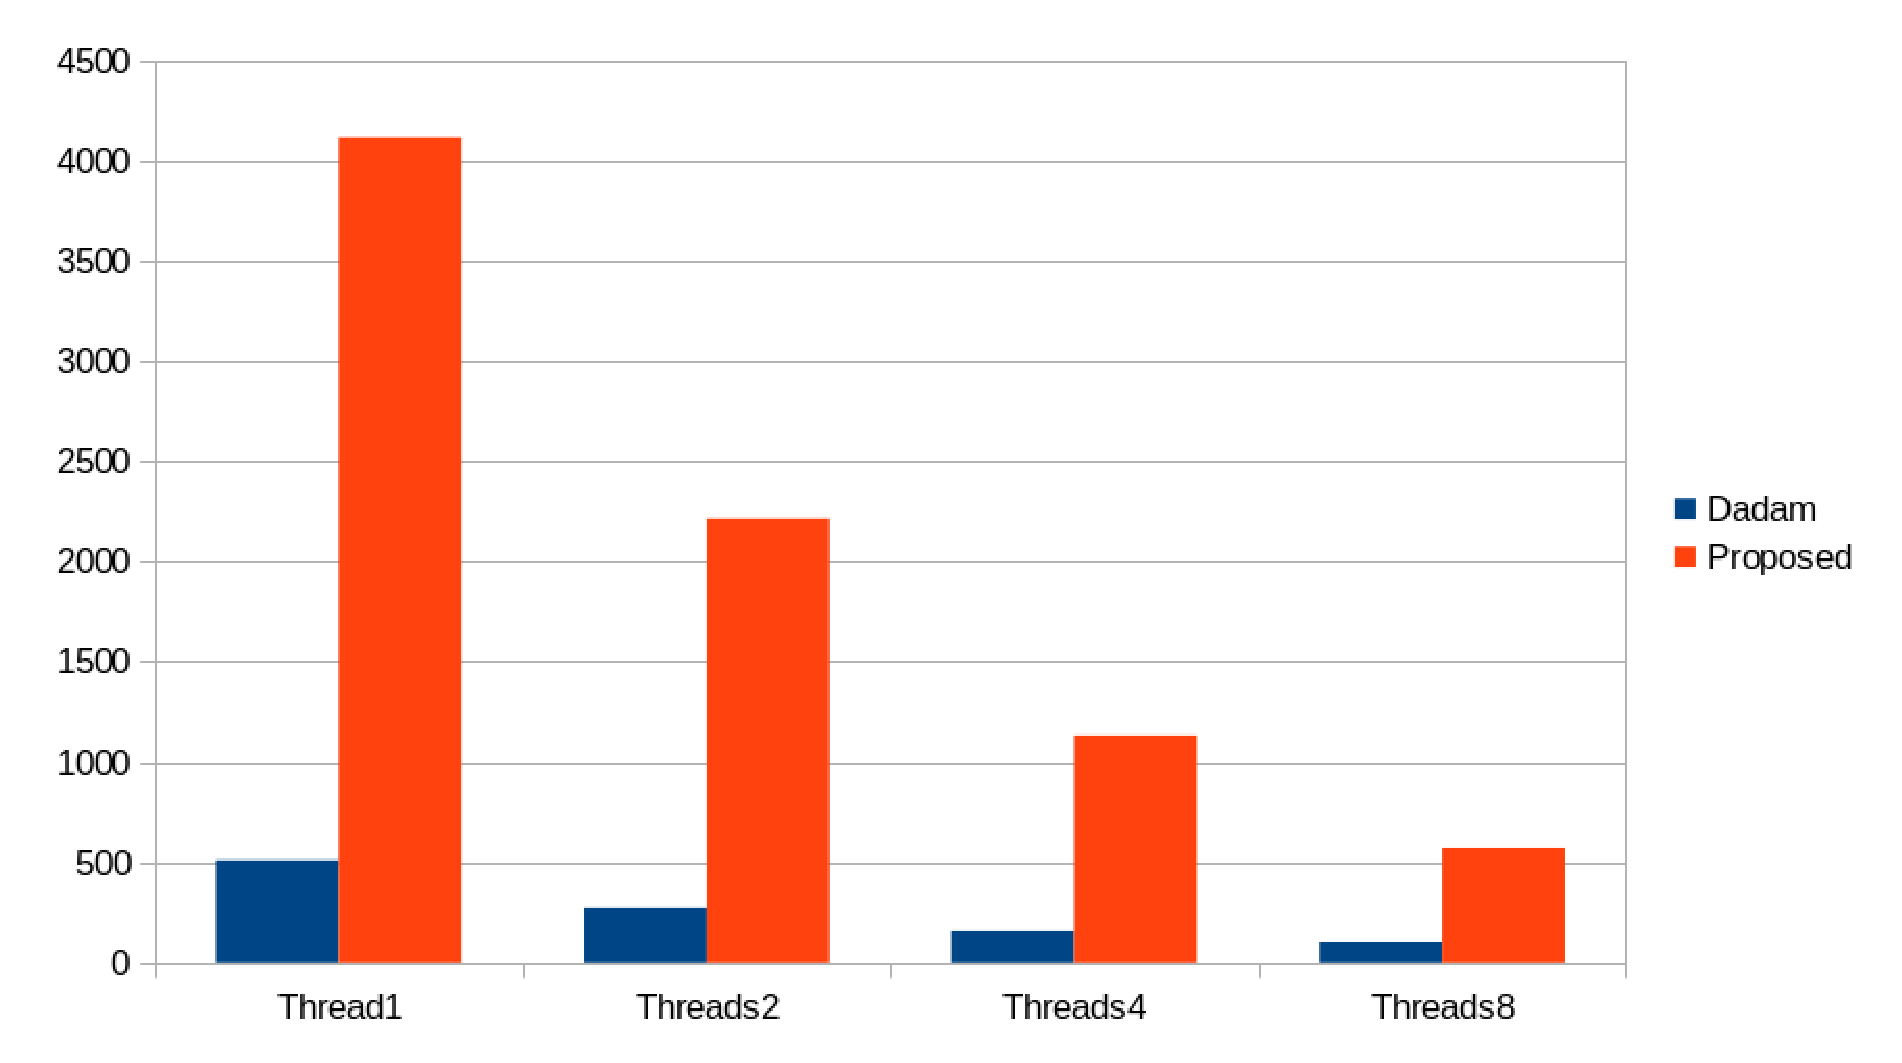
\includegraphics[scale=0.5]{dadam}
\end{figure}


\section{Conclusions\label{sec:Conclusions}}

An innovative method of training artificial neural networks was presented
in this paper. The method consists of two important phases: in the
first phase through a hybrid genetic algorithm, an attempt is made
to identify the optimal interval of initialization and training of
the network parameters and at the second phase the training of the
parameters in the optimal intervals of the first phase is done using
a genetic algorithm. The optimization of the optimal interval in the
first phase is done by using partition rules of the initial interval
that are applied in order. This technique aims to reduce the parameter
search space and then significantly speed up network configuration
training. 

The proposed method was tested on a series of classification and regression
datasets from the relevant literature and the experimental results
seem to be very promising compared to the genetic algorithm procedure.
However, since the method consists of two computational phases, it
is much slower than other training techniques of artificial neural
networks and therefore, the use of parallel processing techniques
is considered necessary.

Future improvements to the proposed method may include the incorporation
of additional global optimization techniques instead of  genetic algorithms,
the usage of more advanced stopping rules and the application of the
method to other types of neural networks such as Radial Basis Function
networks (RBF). 

\subsection*{Compliance with Ethical Standards }

All authors declare that they have no has no conflict of interest. 

\subsection*{Acknowledgments}

The experiments of this research work was performed at the high performance
computing system established at Knowledge and Intelligent Computing
Laboratory, Dept of Informatics and Telecommunications, University
of Ioannina, acquired with the project \textquotedbl Educational
Laboratory equipment of TEI of Epirus\textquotedbl{} with MIS 5007094
funded by the Operational Programme \textquotedbl Epirus\textquotedbl{}
2014-2020, by ERDF and national finds.
\begin{thebibliography}{10}
\bibitem{nn1}C. Bishop, Neural Networks for Pattern Recognition,
Oxford University Press, 1995.

\bibitem{nn2}G. Cybenko, Approximation by superpositions of a sigmoidal
function, Mathematics of Control Signals and Systems \textbf{2}, pp.
303-314, 1989.

\bibitem{nnphysics1}P. Baldi, K. Cranmer, T. Faucett et al, Parameterized
neural networks for high-energy physics, Eur. Phys. J. C \textbf{76},
2016.

\bibitem{nnphysics2}J. J. Valdas and G. Bonham-Carter, Time dependent
neural network models for detecting changes of state in complex processes:
Applications in earth sciences and astronomy, Neural Networks \textbf{19},
pp. 196-207, 2006

\bibitem{nnphysics3}G. Carleo,M. Troyer, Solving the quantum many-body
problem with artificial neural networks, Science \textbf{355}, pp.
602-606, 2017.

\bibitem{nnde1}Y. Shirvany, M. Hayati, R. Moradian, Multilayer perceptron
neural networks with novel unsupervised training method for numerical
solution of the partial differential equations, Applied Soft Computing
\textbf{9}, pp. 20-29, 2009.

\bibitem{nnde2}A. Malek, R. Shekari Beidokhti, Numerical solution
for high order differential equations using a hybrid neural network---Optimization
method, Applied Mathematics and Computation \textbf{183}, pp. 260-271,
2006.

\bibitem{nnagr1}A. Topuz, Predicting moisture content of agricultural
products using artificial neural networks, Advances in Engineering
Software \textbf{41}, pp. 464-470, 2010.

\bibitem{nnagr2}A. Escamilla-Garc�a, G.M. Soto-Zaraz�a, M. Toledano-Ayala,
E. Rivas-Araiza, A. Gast�lum-Barrios, Abraham,Applications of Artificial
Neural Networks in Greenhouse Technology and Overview for Smart Agriculture
Development, Applied Sciences \textbf{10}, Article number 3835, 2020.

\bibitem{nnchem1}Lin Shen, Jingheng Wu, and Weitao Yang, Multiscale
Quantum Mechanics/Molecular Mechanics Simulations with Neural Networks,
Journal of Chemical Theory and Computation \textbf{12}, pp. 4934-4946,
2016.

\bibitem{nnchem2}Sergei Manzhos, Richard Dawes, Tucker Carrington,
Neural network-based approaches for building high dimensional and
quantum dynamics-friendly potential energy surfaces, Int. J. Quantum
Chem. \textbf{115}, pp. 1012-1020, 2015.

\bibitem{nnchem3}Jennifer N. Wei, David Duvenaud, and Al�n Aspuru-Guzik,
Neural Networks for the Prediction of Organic Chemistry Reactions,
ACS Central Science \textbf{2}, pp. 725-732, 2016.

\bibitem{nnecon1}Lukas Falat and Lucia Pancikova, Quantitative Modelling
in Economics with Advanced Artificial Neural Networks, Procedia Economics
and Finance \textbf{34}, pp. 194-201, 2015.

\bibitem{nnecon2}Mohammad Namazi, Ahmad Shokrolahi, Mohammad Sadeghzadeh
Maharluie, Detecting and ranking cash flow risk factors via artificial
neural networks technique, Journal of Business Research \textbf{69},
pp. 1801-1806, 2016.

\bibitem{nncecon3}G. Tkacz, Neural network forecasting of Canadian
GDP growth, International Journal of Forecasting \textbf{17}, pp.
57-69, 2001.

\bibitem{nnmed1}Igor I. Baskin, David Winkler and Igor V. Tetko,
A renaissance of neural networks in drug discovery, Expert Opinion
on Drug Discovery \textbf{11}, pp. 785-795, 2016.

\bibitem{nnmed2}Ronadl Bartzatt, Prediction of Novel Anti-Ebola Virus
Compounds Utilizing Artificial Neural Network (ANN), Chemistry Faculty
Publications \textbf{49}, pp. 16-34, 2018.

\bibitem{nnc}I.G. Tsoulos, D. Gavrilis, E. Glavas, Neural network
construction and training using grammatical evolution, Neurocomputing
\textbf{72}, pp. 269-277, 2008.

\bibitem{bpnn}D.E. Rumelhart, G.E. Hinton and R.J. Williams, Learning
representations by back-propagating errors, Nature \textbf{323}, pp.
533 - 536 , 1986.

\bibitem{bpnn2}T. Chen and S. Zhong, Privacy-Preserving Backpropagation
Neural Network Learning, IEEE Transactions on Neural Networks \textbf{20},
, pp. 1554-1564, 2009.

\bibitem{rpropnn}M. Riedmiller and H. Braun, A Direct Adaptive Method
for Faster Backpropagation Learning: The RPROP algorithm, Proc. of
the IEEE Intl. Conf. on Neural Networks, San Francisco, CA, pp. 586--591,
1993.

\bibitem{rpropnn3}T. Pajchrowski, K. Zawirski and K. Nowopolski,
Neural Speed Controller Trained Online by Means of Modified RPROP
Algorithm, IEEE Transactions on Industrial Informatics \textbf{11},
pp. 560-568, 2015.

\bibitem{rpropnn2}Rinda Parama Satya Hermanto, Suharjito, Diana,
Ariadi Nugroho, Waiting-Time Estimation in Bank Customer Queues using
RPROP Neural Networks, Procedia Computer Science \textbf{ 135}, pp.
35-42, 2018.

\bibitem{key-23}Neural Networks, Procedia Computer Science \textbf{ 135},
pp. 35-42, 2018.

\bibitem{quasinn}B. Robitaille and B. Marcos and M. Veillette and
G. Payre, Modified quasi-Newton methods for training neural networks,
Computers \& Chemical Engineering \textbf{20}, pp. 1133-1140, 1996.

\bibitem{quasinn2}Q. Liu, J. Liu, R. Sang, J. Li, T. Zhang and Q.
Zhang, Fast Neural Network Training on FPGA Using Quasi-Newton Optimization
Method,IEEE Transactions on Very Large Scale Integration (VLSI) Systems
\textbf{26}, pp. 1575-1579, 2018.

\bibitem{geneticnn}F. H. F. Leung, H. K. Lam, S. H. Ling and P. K.
S. Tam, Tuning of the structure and parameters of a neural network
using an improved genetic algorithm, IEEE Transactions on Neural Networks
\textbf{14}, pp. 79-88, 2003

\bibitem{geneticnn2}X. Yao, Evolving artificial neural networks,
Proceedings of the IEEE, 87(9), pp. 1423-1447, 1999.

\bibitem{psonn}C. Zhang, H. Shao and Y. Li, Particle swarm optimisation
for evolving artificial neural network, IEEE International Conference
on Systems, Man, and Cybernetics, , pp. 2487-2490, 2000.

\bibitem{psonn2}Jianbo Yu, Shijin Wang, Lifeng Xi, Evolving artificial
neural networks using an improved PSO and DPSO \textbf{71}, pp. 1054-1060,
2008.

\bibitem{weight_init1}I. Ivanova, M. Kubat, Initialization of neural
networks by means of decision trees, Knowledge-Based Systems \textbf{8},
pp. 333-344, 1995.

\bibitem{weight_init2}J.Y.F. Yam, T.W.S. Chow, A weight initialization
method for improving training speed in feedforward neural network,
Neurocomputing \textbf{30}, pp. 219-232, 2000.

\bibitem{weight_init3}K. Chumachenko, A. Iosifidis, M. Gabbouj, Feedforward
neural networks initialization based on discriminant learning, Neural
Networks \textbf{146}, pp. 220-229, 2022.

\bibitem{weight_decay1}M.D. Shahjahan, M. Kazuyuki, Neural network
training algorithm with possitive correlation, IEEE Trans. Inf \&
Syst. \textbf{88}, pp. 2399-2409, 2005.

\bibitem{weight_decay2}N.K. Treadgold, T.D. Gedeon, Simulated annealing
and weight decay in adaptive learning: the SARPROP algorithm, IEEE
Trans. on Neural Networks \textbf{9}, pp. 662-668, 1998.

\bibitem{weight_decay3}C.S. Leung, K.W. Wong, P.F. Sum, L.W. Chan,
A pruning method for the recursive least squared algorithm, Neural
networks \textbf{14}, pp. 147-174, 2001.

\bibitem{weight_de1}J. lonen, J.K. Kamarainen, J. Lampinen, Differential
Evolution Training Algorithm for Feed-Forward Neural Networks, Neural
Processing Letters \textbf{17}, pp. 93--105, 2003.

\bibitem{weight_de2}M. Baioletti, G. Di Bari, A. Milani, V. Poggioni,
Differential Evolution for Neural Networks Optimization, Mathematics
\textbf{8}, 2020.

\bibitem{weight_aco}K.M. Salama, A.M. Abdelbar, Learning neural network
structures with ant colony algorithms, Swarm Intell \textbf{9}, pp.
229--265, 2015.

\bibitem{weight_nnc}I.G. Tsoulos, D. Gavrilis, E. Glavas, Solving
differential equations with constructed neural networks, Neurocomputing
72, pp. 2385-2391, 2009.

\bibitem{weight_gpu1}M. Mart�nez-Zarzuela, F.J. D�az Pernas, J.F.
D�ez Higuera, M.A. Rodr�guez, Fuzzy ART Neural Network Parallel Computing
on the GPU. In: Sandoval, F., Prieto, A., Cabestany, J., Gra�a, M.
(eds) Computational and Ambient Intelligence. IWANN 2007. Lecture
Notes in Computer Science, vol 4507. Springer, Berlin, Heidelberg,
2007.

\bibitem{weight_gpu2}A.A. Huqqani, E. Schikuta, S. Ye Peng Chen,
Multicore and GPU Parallelization of Neural Networks for Face Recognition,
Procedia Computer Science \textbf{18}, pp. 349-358, 2013.

\bibitem{interval0}E. Hansen and G.W. Walster.Global Optimization
using Interval Analy-sis.Marcel Dekker Inc., New York, 2004.

\bibitem{interval1}M.Cs. Mark�t,Fern�ndezL.G. and CasadoT. Csendes,
New interval methods for constrained global optimization, Mathematical
Programming \textbf{106}, pp. 287-318, 2006.

\bibitem{interval2}A. �ilinskas, and J. �ilinskas, Interval Arithmetic
Based Optimization in Nonlinear Regression, Informatica \textbf{21},
pp. 149-158, 2010.

\bibitem{rnn1}P. Rodriguez, J. Wiles, J.L. Elman, A Recurrent Neural
Network that Learns to Count, Connection Science \textbf{11}, pp.
5-40, 1999.

\bibitem{rnn2}R. Chandra, M. Zhang, Cooperative coevolution of Elman
recurrent neural networks for chaotic time series prediction, Neurocomputing
\textbf{86}, pp. 116-123, 2012.

\bibitem{nn_ann1}A. Yamazaki, M. C. P. de Souto,T. B. Ludermir, Optimization
of neural network weights and architectures for odor recognition using
simulated annealing, In: Proceedings of the 2002 International Joint
Conference on Neural Networks. IJCNN'02 \textbf{1}, pp. 547-552 ,
2002.

\bibitem{nn_ann2}Y. Da, G. Xiurun, An improved PSO-based ANN with
simulated annealing technique, Neurocomputing \textbf{63}, pp. 527-533,
2005.

\bibitem{openmp}L. Dagum, R. Menon, OpenMP: an industry standard
API for shared-memory programming, IEEE Computational Science and
Engineering \textbf{ 5}, pp. 46-55, 1998.

\bibitem{key-6}Z. Michaelewicz, Genetic Algorithms + Data Structures
= Evolution Programs. Springer - Verlag, Berlin, 1996.

\bibitem{kaelo}P. Kaelo, M.M. Ali, Integrated crossover rules in
real coded genetic algorithms, European Journal of Operational Research
\textbf{176}, pp. 60-76, 2007.

\bibitem{powell}M.J.D Powell, A Tolerant Algorithm for Linearly Constrained
Optimization Calculations, Mathematical Programming \textbf{45}, pp.
547-566, 1989. 

\bibitem{Keel}J. Alcal�-Fdez, A. Fernandez, J. Luengo, J. Derrac,
S. Garc�a, L. S�nchez, F. Herrera. KEEL Data-Mining Software Tool:
Data Set Repository, Integration of Algorithms and Experimental Analysis
Framework. Journal of Multiple-Valued Logic and Soft Computing 17,
pp. 255-287, 2011.

\bibitem{appendicitis}Weiss, Sholom M. and Kulikowski, Casimir A.,
Computer Systems That Learn: Classification and Prediction Methods
from Statistics, Neural Nets, Machine Learning, and Expert Systems,
Morgan Kaufmann Publishers Inc, 1991.

\bibitem{australian}J.R. Quinlan, Simplifying Decision Trees. International
Journal of Man-Machine Studies \textbf{27}, pp. 221-234, 1987. 

\bibitem{balance}T. Shultz, D. Mareschal, W. Schmidt, Modeling Cognitive
Development on Balance Scale Phenomena, Machine Learning \textbf{16},
pp. 59-88, 1994.

\bibitem{cleveland1}Z.H. Zhou,Y. Jiang, NeC4.5: neural ensemble based
C4.5,\textquotedbl{} in IEEE Transactions on Knowledge and Data Engineering
\textbf{16}, pp. 770-773, 2004.

\bibitem{cleveland2}R. Setiono , W.K. Leow, FERNN: An Algorithm for
Fast Extraction of Rules from Neural Networks, Applied Intelligence
\textbf{12}, pp. 15-25, 2000.

\bibitem{dermatology}G. Demiroz, H.A. Govenir, N. Ilter, Learning
Differential Diagnosis of Eryhemato-Squamous Diseases using Voting
Feature Intervals, Artificial Intelligence in Medicine. \textbf{13},
pp. 147--165, 1998.

\bibitem{heart}I. Kononenko, E. �imec, M. Robnik-�ikonja, Overcoming
the Myopia of Inductive Learning Algorithms with RELIEFF, Applied
Intelligence \textbf{7}, pp. 39--55, 1997

\bibitem{hayesroth}B. Hayes-Roth, B., F. Hayes-Roth. Concept learning
and the recognition and classification of exemplars. Journal of Verbal
Learning and Verbal Behavior \textbf{16}, pp. 321-338, 1977.

\bibitem{housevotes}R.M. French, N. Chater, Using noise to compute
error surfaces in connectionist networks: a novel means of reducing
catastrophic forgetting, Neural Comput. \textbf{14}, pp. 1755-1769,
2002.

\bibitem{ion1}J.G. Dy , C.E. Brodley, Feature Selection for Unsupervised
Learning, The Journal of Machine Learning Research \textbf{5}, pp
845--889, 2004.

\bibitem{ion2}S. J. Perantonis, V. Virvilis, Input Feature Extraction
for Multilayered Perceptrons Using Supervised Principal Component
Analysis, Neural Processing Letters \textbf{10}, pp 243--252, 1999.

\bibitem{liver} J. Garcke, M. Griebel, Classification with sparse
grids using simplicial basis functions, Intell. Data Anal. \textbf{6},
pp. 483-502, 2002.

\bibitem{mammographic}M. Elter, R. Schulz-Wendtland, T. Wittenberg,
The prediction of breast cancer biopsy outcomes using two CAD approaches
that both emphasize an intelligible decision process, Med Phys. \textbf{34},
pp. 4164-72, 2007.

\bibitem{pageblocks}F. Esposito F., D. Malerba, G. Semeraro, Multistrategy
Learning for Document Recognition, Applied Artificial Intelligence
\textbf{8}, pp. 33-84, 1994. 

\bibitem{parkinsons}M.A. Little, P.E. McSharry, E.J. Hunter, J. Spielman,
L.O. Ramig, Suitability of dysphonia measurements for telemonitoring
of Parkinson's disease. IEEE Trans Biomed Eng. \textbf{56}, pp. 1015-1022,
2009.

\bibitem{pima}J.W. Smith, J.E. Everhart, W.C. Dickson, W.C. Knowler,
R.S. Johannes, Using the ADAP learning algorithm to forecast the onset
of diabetes mellitus, In: Proceedings of the Symposium on Computer
Applications and Medical Care IEEE Computer Society Press, pp.261-265,
1988.

\bibitem{popfailures}D.D. Lucas, R. Klein, J. Tannahill, D. Ivanova,
S. Brandon, D. Domyancic, Y. Zhang, Failure analysis of parameter-induced
simulation crashes in climate models, Geoscientific Model Development
\textbf{6}, pp. 1157-1171, 2013.

\bibitem{regions}N. Giannakeas, M.G. Tsipouras, A.T. Tzallas, K.
Kyriakidi, Z.E. Tsianou, P. Manousou, A. Hall, E.C. Karvounis, V.
Tsianos, E. Tsianos, A clustering based method for collagen proportional
area extraction in liver biopsy images (2015) Proceedings of the Annual
International Conference of the IEEE Engineering in Medicine and Biology
Society, EMBS, 2015-November, art. no. 7319047, pp. 3097-3100. 

\bibitem{saheart}T. Hastie, R. Tibshirani, Non-parametric logistic
and proportional odds regression, JRSS-C (Applied Statistics) \textbf{36},
pp. 260--276, 1987.

\bibitem{segment}M. Dash, H. Liu, P. Scheuermann, K. L. Tan, Fast
hierarchical clustering and its validation, Data \& Knowledge Engineering
\textbf{44}, pp 109--138, 2003.

\bibitem{wdbc}W.H. Wolberg, O.L. Mangasarian, Multisurface method
of pattern separation for medical diagnosis applied to breast cytology,
Proc Natl Acad Sci U S A. \textbf{87}, pp. 9193--9196, 1990.

\bibitem{wine1}M. Raymer, T.E. Doom, L.A. Kuhn, W.F. Punch, Knowledge
discovery in medical and biological datasets using a hybrid Bayes
classifier/evolutionary algorithm. IEEE transactions on systems, man,
and cybernetics. Part B, Cybernetics : a publication of the IEEE Systems,
Man, and Cybernetics Society, \textbf{33} , pp. 802-813, 2003.

\bibitem{wine2}P. Zhong, M. Fukushima, Regularized nonsmooth Newton
method for multi-class support vector machines, Optimization Methods
and Software \textbf{22}, pp. 225-236, 2007.

\bibitem{zoo}M. Koivisto, K. Sood, Exact Bayesian Structure Discovery
in Bayesian Networks, The Journal of Machine Learning Research\textbf{
5}, pp. 549--573, 2004.

\bibitem{key-20}R.G. Andrzejak, K. Lehnertz, F. Mormann, C. Rieke,
P. David, and C. E. Elger, Indications of nonlinear deterministic
and finite-dimensional structures in time series of brain electrical
activity: Dependence on recording region and brain state, Phys. Rev.
E \textbf{64}, pp. 1-8, 2001.

\bibitem{abalone}W. J Nash, T.L. Sellers, S.R. Talbot, A.J. Cawthor,
W.B. Ford, The Population Biology of Abalone (\_Haliotis\_ species)
in Tasmania. I. Blacklip Abalone (\_H. rubra\_) from the North Coast
and Islands of Bass Strait, Sea Fisheries Division, Technical Report
No. 48 (ISSN 1034-3288), 1994.

\bibitem{airfoil}T.F. Brooks, D.S. Pope, A.M. Marcolini, Airfoil
self-noise and prediction. Technical report, NASA RP-1218, July 1989. 

\bibitem{Stat}J.S. Simonoff, Smooting Methods in Statistics, Springer
- Verlag, 1996.

\bibitem{concrete}I.Cheng Yeh, Modeling of strength of high performance
concrete using artificial neural networks, Cement and Concrete Research.
\textbf{28}, pp. 1797-1808, 1998. 

\bibitem{key23}D. Harrison and D.L. Rubinfeld, Hedonic prices and
the demand for clean ai, J. Environ. Economics \& Management \textbf{5},
pp. 81-102, 1978.

\bibitem{key21}J.S. Simonoff, Smooting Methods in Statistics, Springer
- Verlag, 1996.

\bibitem{pydataset}R.D. King, S. Muggleton, R. Lewis, M.J.E. Sternberg,
Proc. Nat. Acad. Sci. USA \textbf{89}, pp. 11322--11326, 1992. 

\bibitem{Adam}D. P. Kingma, J. L. Ba, ADAM: a method for stochastic
optimization, in: Proceedings of the 3rd International Conference
on Learning Representations (ICLR 2015), pp. 1--15, 2015.

\bibitem{fcn}Grzegorz Klima, Fast Compressed Neural Networks, available
from \url{http://fcnn.sourceforge.net/}.

\bibitem{neat}K. O. Stanley, R. Miikkulainen, Evolving Neural Networks
through Augmenting Topologies, Evolutionary Computation \textbf{10},
pp. 99-127, 2002.
\end{thebibliography}

\end{document}
